% Author: Dominik Harmim <harmim6@gmail.com>


\documentclass[%
    10pt, xcolor=pdflatex, hyperref={unicode}, aspectratio=169%
]{beamer}


\usepackage{newcent}
\usepackage[utf8]{inputenc}
\usepackage[british]{babel}
\usepackage[T1]{fontenc}
\usepackage{xcolor}
\usepackage{listings}

\definecolor{bluekeywords}{rgb}{.13, .13, 1}
\definecolor{greencomments}{rgb}{0, .5, 0}
\definecolor{redstrings}{rgb}{.9, 0, 0}
\lstset{
    basicstyle=\ttfamily,
    keywordstyle=\color{bluekeywords},
    commentstyle=\color{greencomments},
    stringstyle=\color{redstrings},
    backgroundcolor=\color{white},
    language=C++,
    tabsize=2,
    escapeinside={<@}{@>},
    frame=trBL,
    columns=fullflexible,
    showstringspaces=true,
    keepspaces=true,
    showspaces=false,
    showtabs=false,
    breaklines=true,
    breakatwhitespace=true
}


%%%%%%%%%%%%%%%%%%%%%%%%%%%%%%%%%%%%%%%%%%%%%%%%%%%%%%%%%%%%%%%%%%%%%%%%%%%%%%%%
\usetheme{FIT}

\title[%
    Advanced Static Analysis of Atomicity in Concurrent Programs through
    Facebook Infer%
]{%
    Advanced Static Analysis of Atomicity in Concurrent Programs through
    Facebook Infer%
}
\subtitle{\texorpdfstring{SEP\,---\,Term Project}{SEP - Term Project}}

\author{\texorpdfstring{%
    Dominik Harmim \\
    \footnotesize{Supervisor: prof. Ing. Tomáš Vojnar, Ph.D.}%
}{Dominik Harmim; Supervisor: prof. Ing. Tomáš Vojnar, Ph.D.}}

\institute{%
    xharmi00@stud.fit.vutbr.cz \\
    Brno University of Technology, Faculty of Information Technology%
}

\date{\today}
%%%%%%%%%%%%%%%%%%%%%%%%%%%%%%%%%%%%%%%%%%%%%%%%%%%%%%%%%%%%%%%%%%%%%%%%%%%%%%%%


\begin{document}


%%%%%%%%%%%%%%%%%%%%%%%%%%%%%%%%%%%%%%%%%%%%%%%%%%%%%%%%%%%%%%%%%%%%%%%%%%%%%%%%
\section{Title Page}
\frame[plain]{\titlepage}


%%%%%%%%%%%%%%%%%%%%%%%%%%%%%%%%%%%%%%%%%%%%%%%%%%%%%%%%%%%%%%%%%%%%%%%%%%%%%%%%
\section{Motivation}
\begin{frame}[fragile]{Motivation}
    \begin{itemize}
        \item
            Detecting and checking desired \alert{atomicity of call sequences}:
            \smallskip
            \begin{itemize}\setlength\itemsep{1em}
                \item
                    Often required in \emph{concurrent programs}.

                \item
                    \alert{Violation} may cause \emph{nasty errors}.
            \end{itemize}
    \end{itemize}

    \medskip

    \begin{columns}
        \begin{column}{.6 \linewidth}
            \centering
\begin{lstlisting}
void invoke(char *method) {
    <@\texttt{\ldots}@>
    if (server.<@\textbf{is\_registered}@>(method)) {
        server.<@\textbf{invoke}@>(method);
    }
    <@\texttt{\ldots}@>
}
\end{lstlisting}
        \end{column}

        \begin{column}{.4 \linewidth}
            \centering

            The \emph{sequence} of \texttt{\textbf{is\_registered}} and
            \texttt{\textbf{invoke}} should be \alert{executed atomically}.

            \medskip

            {\footnotesize%
                If \emph{not locked}, the method can be
                unregistered by a~\emph{concurrent thread}.%
            }
        \end{column}
    \end{columns}
\end{frame}


%%%%%%%%%%%%%%%%%%%%%%%%%%%%%%%%%%%%%%%%%%%%%%%%%%%%%%%%%%%%%%%%%%%%%%%%%%%%%%%%
\section{Facebook Infer}
\begin{frame}{Facebook Infer}
    \begin{columns}
        \begin{column}{1 \linewidth}
            \begin{itemize}
                \item
                    An open-source \alert{static analysis framework}
                    for \emph{interprocedural analyses}.
                    \smallskip
                    \begin{itemize}\setlength\itemsep{1em}
                        \item
                            Based on \alert{abstract interpretation}.
                    \end{itemize}
            \end{itemize}
        \end{column}

        \hfill
    \end{columns}

    \begin{columns}
        \begin{column}{.55 \linewidth}
            \begin{itemize}\setlength\itemsep{2em}
                \item
                    Highly \alert{scalable}:
                    \smallskip
                    \begin{itemize}\setlength\itemsep{1em}
                        \item
                            Follows principles of \emph{compositionality}.

                        \item
                            Computes function \emph{summaries}
                            \alert{bottom-up} on call trees.
                    \end{itemize}

                \item
                    Supports C, C++, Java, Obj-C (and C\#).
            \end{itemize}
        \end{column}

        \begin{column}{.45 \linewidth}
            \centering
            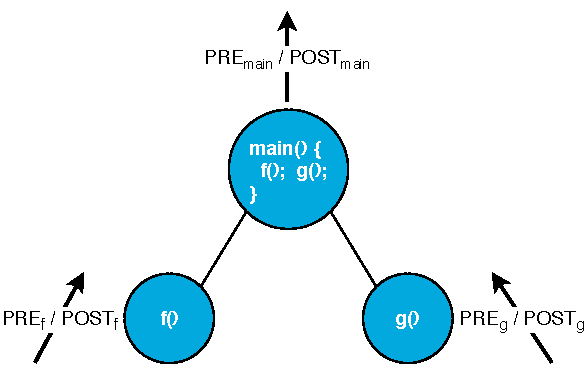
\includegraphics[width=1 \linewidth]{img/infer.pdf}
        \end{column}
    \end{columns}
\end{frame}


%%%%%%%%%%%%%%%%%%%%%%%%%%%%%%%%%%%%%%%%%%%%%%%%%%%%%%%%%%%%%%%%%%%%%%%%%%%%%%%%
\section{Atomer: Atomicity Violations Analyser}
\begin{frame}{Atomer: Atomicity Violations Analyser}
    \begin{itemize}\setlength\itemsep{2em}
        \item
            A~\alert{Facebook Infer plugin} created within
            the bachelor's thesis:
            \medskip
            \begin{thebibliography}{1}
                \bibitem[harmimBP]{harmimBP}
                \textsc{Harmim, D.} \textit{Static Analysis Using Facebook
                Infer to Find Atomicity Violations}. Brno, 2019. Bachelor's
                thesis. Brno University of Technology, Faculty of Information
                Technology. Supervisor \textsc{Vojnar, T.}
            \end{thebibliography}

        \item
            \textbf{Assumption}: \alert{Call sequences} executed
            \emph{atomically once} should (probably) be executed
            \emph{always atomically}.

        \item
            Implemented for \emph{C}~programs that use \emph{PThread locks}.
            
        \item
            Limited \alert{scalability} on extensive codebases.
            
        \item
            Reports many \alert{false alarms} when analysing \emph{real-life}
            code.
    \end{itemize}
\end{frame}


%%%%%%%%%%%%%%%%%%%%%%%%%%%%%%%%%%%%%%%%%%%%%%%%%%%%%%%%%%%%%%%%%%%%%%%%%%%%%%%%
\section{High-Level Analysis Process (with Extensions)}
\begin{frame}{High-Level Analysis Process (with Extensions)}
    \centering
    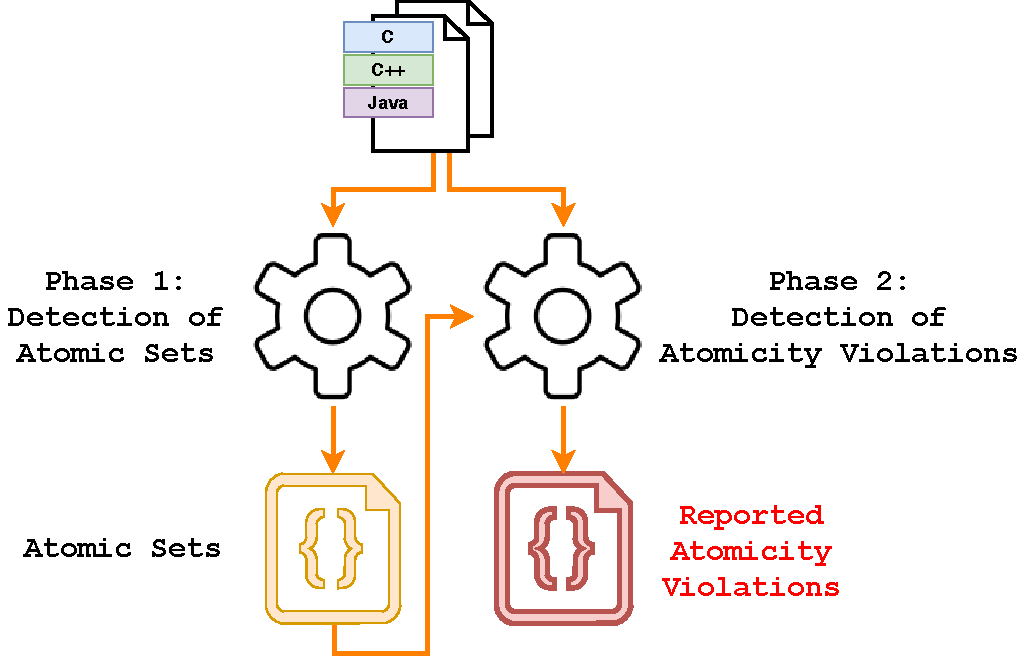
\includegraphics[width=.8 \linewidth]{img/analyser-proposal-sets.pdf}
\end{frame}


%%%%%%%%%%%%%%%%%%%%%%%%%%%%%%%%%%%%%%%%%%%%%%%%%%%%%%%%%%%%%%%%%%%%%%%%%%%%%%%%
\section{Two Phases of the Analysis (Improved Scalability)}
\begin{frame}[fragile]{Two Phases of the Analysis (Improved Scalability)}
    \begin{columns}
        \begin{column}[T]{.55 \linewidth}
            \begin{enumerate}
                \item
                    Detection of \alert{atomic call sets}.
            \end{enumerate}

            \begin{itemize}
                \item
                    \emph{Approximates} \alert{sequences by sets}.

                \item
                    \textbf{Summaries}: (\textcolor{brown}{set of all
                    calls}, \textcolor{magenta}{set of atomic call sets})
            \end{itemize}

\begin{lstlisting}
void f() {
    <@\texttt{\textcolor{red}{\textbf{lock}}}@>(L); 
    x(); y(); z();
    <@\texttt{\textcolor{red}{\textbf{unlock}}}@>(L);
    a();
    <@\texttt{\textcolor{red}{\textbf{lock}}}@>(L); 
    z(); y(); x(); 
    <@\texttt{\textcolor{red}{\textbf{unlock}}}@>(L);
}
\end{lstlisting}

            \textbf{\texttt{\footnotesize
                \alert{$ Summary_\mathtt{f} $}:\,%
                (\textcolor{brown}{\{a,~x,~y,~z\}},
                \textcolor{magenta}{\{\{x,~y,~z\}\}})
            }}
            
            \textcolor{gray}{\texttt{\scriptsize
                $ Summary_\mathtt{f}^\prime $:\,%
                (\textcolor{brown}{(x,~y,~z,~a)},
                \textcolor{magenta}{\{(x,~y,~z), (z,~y,~x)\}})
            }}
        \end{column}

        \begin{column}[T]{.45 \linewidth}
            \begin{enumerate}\setcounter{enumi}{1}
                \item
                    Detection of \alert{atomicity violations}.
            \end{enumerate}

            \begin{itemize}
                \item
                    Looks for \emph{non-atomic pairs of calls}
                    assumed to \alert{run atomically}.

                \item
                    \textbf{Summaries}: (\textcolor{orange}{set of
                    first calls}, \textcolor{violet}{set of last
                    calls}, \textcolor{red}{set of atomicity
                    violations})
            \end{itemize}

\begin{lstlisting}
void g() {
    a();
    <@\texttt{\textcolor{red}{\textbf{x}}}@>(); <@\texttt{\textcolor{red}{\textbf{y}}}@>();
    b();
}
\end{lstlisting}

            \textbf{\texttt{\scriptsize
                $ AtomPairs_\mathtt{f} $:\,%
                \{(x,~y), (x,~z), (y,~x), (y,~z), \\ \hspace{6em}
                (z,~x), (z,~y)\}
            }}
            
            \textcolor{gray}{\texttt{\scriptsize
                $ AtomPairs_\mathtt{f}^\prime $:\,%
                \{(x,~y), (y,~z), (z,~y), (y,~x)\}
            }}
            \textbf{\texttt{\footnotesize
                \alert{$ Summary_\mathtt{g} $}:\,%
                (\textcolor{orange}{\{a\}},
                \textcolor{violet}{\{b\}},
                \textcolor{red}{\{(x,~y)\}})
            }}
        \end{column}
    \end{columns}
\end{frame}


%%%%%%%%%%%%%%%%%%%%%%%%%%%%%%%%%%%%%%%%%%%%%%%%%%%%%%%%%%%%%%%%%%%%%%%%%%%%%%%%
\section{Precision Enhancements and Other Extensions}
\begin{frame}{Precision Enhancements and Other Extensions}
    \begin{itemize}\setlength\itemsep{2.5em}
        \item
            Support for \alert{C++ and Java}:
            \smallskip
            \begin{itemize}\setlength\itemsep{1em}
                \item
                    \textbf{C++}: \texttt{std::mutex, std::lock,
                    std::lock\_guard, \ldots}

                \item
                    \textbf{Java}: \emph{monitors} (\texttt{synchronized})%
                    \texttt{, Lock, ReentrantLock, \ldots}
            \end{itemize}

        \item
            Distinguishing \alert{multiple (nested) locks} used:
            \smallskip
            \begin{itemize}\setlength\itemsep{1em}
                \item
                    \emph{Approximates lock objects} using \alert{syntactic
                    access paths}\,---\,a~representation of \emph{heap
                    locations} via the paths used to access them.
            \end{itemize}
            
        \item
            \alert{Parametrisation} of the analysis by a~user:
            \smallskip
            \begin{itemize}\setlength\itemsep{1em}
                \item
                    ignore \emph{generic functions}/concentrate on
                    \emph{critical functions},
                    
                \item
                    limit \emph{the number of calls} or \emph{the depth of
                    analysing nested calls} in \alert{critical sections}.
            \end{itemize}
    \end{itemize}
\end{frame}


%%%%%%%%%%%%%%%%%%%%%%%%%%%%%%%%%%%%%%%%%%%%%%%%%%%%%%%%%%%%%%%%%%%%%%%%%%%%%%%%
\section{Experimental Evaluation}
\begin{frame}{Experimental Evaluation}
    \begin{itemize}\setlength\itemsep{3em}
        \item
            The \alert{correctness} of the extensions was verified on
            \emph{hand-crafted} programs.

        \item
            \alert{Real-life Java} programs\,---\,\emph{Apache Cassandra}
            and \emph{Tomcat} ($ \sim $200k LOC).
            \bigskip
            \begin{itemize}\setlength\itemsep{2em}
                \item
                    Successfully \alert{rediscovered} \emph{already fixed
                    reported real bugs}.

                \item
                    So far quite some \alert{false alarms}\,---\,need
                    to further increase \emph{accuracy}.
            \end{itemize}
    \end{itemize}
\end{frame}


%%%%%%%%%%%%%%%%%%%%%%%%%%%%%%%%%%%%%%%%%%%%%%%%%%%%%%%%%%%%%%%%%%%%%%%%%%%%%%%%
\section{Summary}
\begin{frame}{Summary}
    \textbf{\alert{Extensions} for \emph{Atomer}:}
    \medskip
    \begin{itemize}\setlength\itemsep{.5em}
        \item
            \emph{Proposed} and \emph{implemented} extensions for Atomer:
            
            \begin{itemize}
                \item
                    approximation of sequences by sets, support for C++ and
                    Java, distinguishing multiple locks, parametrisation of
                    the analysis.
            \end{itemize}
            
        \item
            Successfully \emph{tested} and \emph{experimentally evaluated}.
            
        \item
            Experiments with \emph{real-life programs}.
    \end{itemize}

    \bigskip

    \textbf{Future goals:}
    \medskip
    \begin{itemize}\setlength\itemsep{.5em}
        \item
            Further analysis of \emph{real-life programs} with
            an effort to find and report \alert{new bugs}.

        \item
            Increase \alert{accuracy}/reduce the number of \alert{false
            alarms}:

            \begin{itemize}\setlength\itemsep{.5em}
                \item
                    Support for \emph{interprocedural locks}.

                \item
                    Combination with \emph{dynamic analysis}.

                \item
                    \emph{Statistic ranking} of atomic functions/reported
                    errors.
            \end{itemize}
    \end{itemize}
\end{frame}


\end{document}
